\section{Effective and efficient tracking in a floating disc}
%\section{Tracking in a circular area}
\label{sec:circle}

{\ldrh is a one-pass trajectory tracking algorithm, having linear time and constant space complexities, and suffering in effectiveness (compression ratios).
Observing the recently trajectory simplification algorithm using \sed, named  \cised, is also one-pass (which is important for a trajectory tracking algorithm that is supposed to run on mobile devices), and at the same time, it has a good effectiveness (compression ratios), these inspire us to develop an efficient and effective trajectory tracking algorithm using \sed.}


%\subsection{Spatio-temporal cones and their usage in trajectory simplification}
\subsection{Spatio-temporal cones}
\cised uses a local synchronous distance checking approach based on a concept of \textit{spatio-temporal cone}, defined in a 3D Cartesian coordinate system whose $x$-axis, $y$-axis and $t$-axis are longitude, latitude and time, respectively, that converts the \sed distance tolerance into cones intersection for testing the successive points. This mechanism is potential to be extended for trajectory tracking with good effectiveness and efficiency.

\stitle{Spatio-temporal cone (\cone{}) \cite{Lin:Cised}}. 
Given a start point $P_s$ of sub-trajectory $\dddot{\mathcal{T}}_s[P_s, \ldots, P_{s+k}]$ and an error bound $\epsilon$, the spatio-temporal cone (or simply \textit{cone}) of a data point $P_{s+i}$ ($1\le i\le k$) in $\dddot{\mathcal{T}_s}$ \wrt $P_s$ and $\epsilon$, denoted as \cone{(P_s, P_{s+i}, \epsilon)}, or \cone{_{s+i}} in short, is an oblique circular cone such that point $P_s$ is its apex and the synchronous circle $\mathcal{O}(P_{s+i}, \epsilon)$ of point $P_{s+i}$, or \circle{_{s+i}} in short, a circle on the plane $P.t-P_{s+i}.t = 0$ such that $P_{s+i}$ is its center and $\epsilon$ is its radius, is its base (Figure~\ref{fig:cis}).

\eat{%%%%%%%%%%%
	\begin{example}
		\label{exm-circles-cones}
		Figure~\ref{fig:cis} shows 
		(1) two synchronous circles, \circle{(P_{s+i}, \epsilon)} of point $P_{s+i}$ and \circle{(P_{s+k}, \epsilon)} of point $P_{s+k}$.
		It is easy to see that for any point in the area of a circle \circle{(P_{s+i}, \epsilon)}, its distance to $P_{s+i}$ is not greater than $\epsilon$, 
		and (2) two example spatio-temporal cones, \cone{(P_s, P_{s+i}, \epsilon)} {(purple)} and \cone{(P_s, P_{s+k}, \epsilon)} (red), with the same apex $P_s$ and error bound $\epsilon$. %\eop
	\end{example}
}%%%%%%%%%%%

%Note that in this definition, a \emph{synchronous circle} $\mathcal{O}(P_i, \epsilon)$ is only defined by a central point $P_i$ and a constant $\epsilon$. Indeed, it is nothing to do with any start point $P_s$ or end point $P_e$.


%\textcolor{blue}{We define \textit{synchronous circles and Spatio-temporal cones} in a \emph{x-y-t} 3D coordinate system, and build the connection between \textit{synchronous circles} and \textit{synchronous distances}.}



\begin{figure}[tb!]
	\centering
	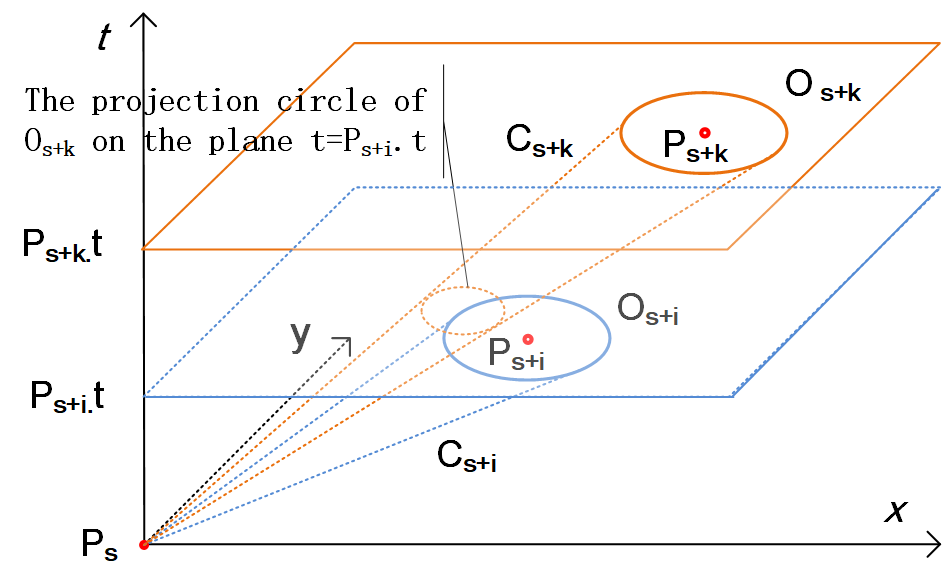
\includegraphics[scale=0.88]{figures/Fig-CIS.png}
	\vspace{-2ex}
	\caption{\small Examples of spatio-temporal cones in a 3D Cartesian coordinate system taking point $P_s$ as the origin, where (1) $P_{s+i}$ and $P_{s+k}$ are two points, (2) \circle{_{s+i}} and \circle{_{s+k}} are two synchronous circles, (3) \cone{_{s+i}} and \cone{_{s+k}} are two spatio-temporal cones.}
	\vspace{-1ex}
	\label{fig:cis}
\end{figure}
%, (4) $Q$ is a point in synchronous circle \circle{_{s+k}}, and (5) $P'_{s+i}$ is the intersection point of line $\protect\overline{P_sQ}$ and synchronous circle \circle{_{s+i}}

Based on the spatio-temporal cones, authors in \cite{Lin:Cised} prove that the \sed distance tolerance can be checked by finding the common intersection of spatio-temporal cones (half-$\epsilon$) built from points of a sub-trajectory $[P_s,...,P_{s+k}]$, \ie ``{given a sub-trajectory $[P_s,...,P_{s+k}]$ and an error bound $\epsilon$, $sed(P_{s+i}, \overline{P_sP_{s+k}})\le \epsilon$ for each $i \in [1,k]$ if  $\bigsqcap_{i=1}^{k}$\cone{(P_s, P_{s+i}, \epsilon/2)} $\ne \{P_s\}$}''.
In other words, if these cones do have a common intersection, then line segment $\overline{P_sP_{s+k}}$ is able to represent the sub-trajectory. And for efficiency consideration, \cised projects those cones on a plane, \eg plane $t=P_{s+1}.t$, so as to convert the checking of cones intersection into a much simpler way, \ie~\textit{checking of circles intersection on the plane} (Figure~\ref{fig:cis}).
For the same reason, a circle is further approximated by its inscribe \emph{regular polygon} $\mathcal{R}$ and the intersecting of circles is approximated by the intersecting of these polygons, which can be computed in linear time.
%
%Note that though the cone intersection approach outperform the counterpart of \ldr and \ldrh, it is still not introduced to trajectory tracking.

\eat{%%%%%%%%%%%%%%%%%% Delete because of the page limitation.
	Figure~\ref{fig:cised} is a running example of \cised. In this case, it outperforms \ldrh in terms of compression ratio.
	
	\begin{figure}[tb!]
		\centering
		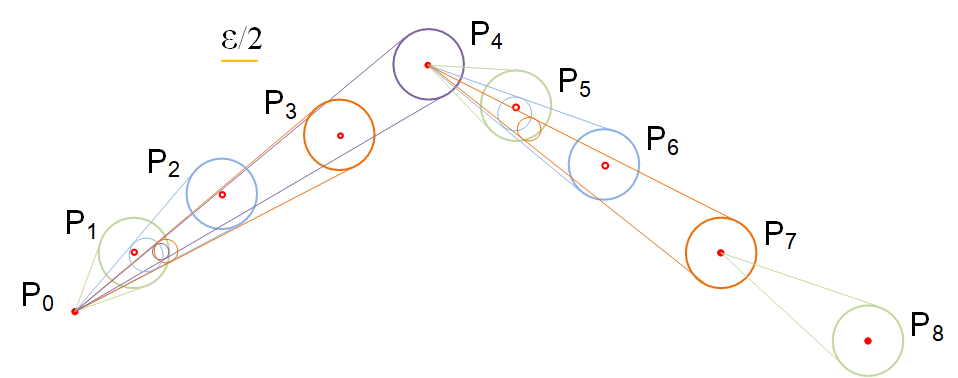
\includegraphics[scale=0.9]{figures/Fig-CISED-SH.png}
		\vspace{-1ex}
		\caption{\small A running example of \cised. In the first section, cones are projected on plane $P_1.t$, where (1) the projection circles of \circle{_{1}},\circle{_{2}},\circle{_{3}} and \circle{_{4}} have common intersection, and (2) it does not intersected with the projection circle of \circle{_{5}}. Thus, $P_4$ is output, and it serves as the new start point of the next section. Finally, the same trajectory is simplified to four points $\{P_0, P_4, P_7, P_8\}$.}
		\vspace{-2ex}
		\label{fig:cised}
	\end{figure}
}%%%%%%%%%%%%%%%%%%%%%%


\subsection{Tracking with spatio-temporal cones}

In this section, we will first show that the counterpart of \ldrh is just a special case of, and has a worse effectiveness in terms of compression ratio than the approaches based on spatio-temporal cone (even it uses a half-$\epsilon$ cone), thus, the latter is obviously a more effective way to develop trajectory tracking algorithms. Then, we further extend the half-$\epsilon$ cone used in \cised to a full-$\epsilon$ cone so as to get an even better effectiveness.



\begin{proposition}
\label{theo-ldrh-cised}
Given a sub-trajectory $\dddot{\mathcal{T}}_s[P_s,...,P_{s+k}]$ and an error bound $\epsilon$, if $\dddot{\mathcal{T}}_s$ can be represented by line segment $\overline{P_sP_{s+k}}$ through algorithm \ldrh, then it can also be represented by approaches based on spatio-temporal cones.
\end{proposition}

\begin{proof}
If $\dddot{\mathcal{T}}_s$ can be represented by line segment $\overline{P_sP_{s+k}}$ by algorithm \ldrh, then we have $|P_{s+i}P'_{s+i}| < \epsilon/2$ for each $i \in (0, k)$, where $P'_{s+i}$ is the expected position (synchronized point) of $P_{s+i}$ \wrt the initial velocity $\vv{v}$ of \ldrh.
From the view of the ``x-y-t'' 3D space, $\vv{v}$ must be in the common intersection of  $\bigsqcap_{i=1}^{k}$\cone{(P_s, P_{s+i}, \epsilon/2)}, in other words, we have $\bigsqcap_{i=1}^{k}$\cone{(P_s, P_{s+i}, \epsilon/2)} $\ne \{P_s\}$, meaning this sub-trajectory can be represented by approaches based on the spatio-temporal cones.
\end{proof}

Proposition \ref{theo-ldrh-cised} tells that (1) {approaches based on the spatio-temporal cone are also applicable to do trajectory tracking in a circular area}, and (2) \ldrh is just a special case of and has a worse effectiveness than approaches based on spatio-temporal cones. \ldrh assumes an initial velocity before the simplification or tracking of a sub-trajectory, while the spatio-temporal cone based methods do not, instead, it has an ability to find out the potentially feasible velocities to fit the movement of the object when it simplifies the sub-trajectory. Thus, the latter is sure a more effective way to develop one-pass trajectory tracking algorithms. 
%
Moreover, observe that the half-$\epsilon$ cone in the above is still a little conservative, we next extend it to a full-$\epsilon$ cone.% plus certain constrain to get an even better effectiveness.


\begin{proposition}
	\label{theo-full-cone}
	Given a sub-trajectory $[P_s,...,P_{s+k}]$ and an error bound $\epsilon$, $sed(P_{s+i}, \overline{P_sP_{s+k}})\le \epsilon$ for each $i \in [1,k]$ if $\overline{P_sP_{s+k}}$ passes through $\bigsqcap_{i=1}^{k-1}$\cone{(P_s, P_{s+i}, \epsilon)} - \{$P_s$\}.
\end{proposition}

\begin{proof}
Let $P'_{s+i}$ be the intersection point of line segment $\overline{P_sP_{s+k}}$ and plane $t = P_{s+i}.t,~i\in (0,k)$, indeed, $P_{s+i}$ is the synchronized point of $P_{s+i}$ \wrt line segment $\overline{P_sP_{s+k}}$. 
Because $\overline{P_sP_{s+k}}$ passes through $\bigsqcap_{i=1}^{k-1}$\cone{(P_s, P_{s+i}, \epsilon)} - \{$P_s$\}, $P'_{s+i}$ must be inside of the synchronous circle of $P_{s+i}$ on the plane. Thus we have $|P_{s+i}P'_{s+i}|<\epsilon$, \ie $sed(P_{s+i}, \overline{P_sP_{s+k}})|<\epsilon$.
\end{proof}

Proposition \ref{theo-full-cone} tells that full-$\epsilon$ spatio-temporal cones, with a constrain that the line segment $\overline{P_sP_{s+i}}$ passes through the common intersection of all the preview cones, can also be used in trajectory simplification and/or tracking. Thus we get two ways of trajectory tracking in a circle. The question is, which one is the better?

\begin{proposition}
	\label{theo-cone-vs}
	Given a sub-trajectory $[P_s,...,P_{s+k}]$ and an error bound $\epsilon$, if $\bigsqcap_{i=1}^{k}$\cone{(P_s, P_{s+i}, \epsilon/2)} $\ne \{P_s\}$, then $\overline{P_sP_{s+k}}$ passes through $\bigsqcap_{i=1}^{k-1}$\cone{(P_s, P_{s+i}, \epsilon)}-$\{P_s\}$; and the opposite is not necessarily true.
\end{proposition}

\begin{proof}
(1) If $\bigsqcap_{i=1}^{k}$\cone{(P_s, P_{s+i}, \epsilon/2)} $\ne \{P_s\}$, then $sed(P_{s+i}, P_sP_{s+k}) <\epsilon$ for each $i \in [1,k]$. 
The intersection point  $P'_{s+i}$ of line segment $P_s P_{s+k}$ and plane $t = P_{s+i}.t$ is the synchronized point of $P_{s+i}$ \wrt $P_s P_{s+k}$, such that $|P_{s+i}P'_{s+i]}| < \epsilon$. Hence for each $i \in [1,k]$, $P'_{s+i}$ falls in the synchronous circle of $P_{s+i}$ on the plane, meaning $\overline{P_sP_{s+k}}$ passes through the common intersection of the preview cones $\bigsqcap_{i=1}^{k-1}$\cone{(P_s, P_{s+i}, \epsilon)}-$\{P_s\}$.
%
(2) If line segment $\overline{P_sP_{s+k}}$ passes through the common intersection $\bigsqcap_{i=1}^{k-1}$\cone{(P_s, P_{s+i}, \epsilon)} - \{$P_s$\}, then, suppose there is $i$ and $j$ ($i<j<k$) such that $P^{s+j}_{s+i}$ and $P^{s+k}_{s+i}$ are the intersection points of $\overline{P_sP_{s+j}}$ and $\overline{P_sP_{s+k}}$ with the plane $t = P_{s+i}.t$, respectively, we have $0 \le |P_{s+i}P^{s+k}_{s+i}|<\epsilon$ and $0 \le |P^{s+j}_{s+i}P^{s+k}_{s+i}|<\epsilon$, meaning $0 \le |P_{s+i}P^{s+j}_{s+i}|<2\epsilon$, \ie~$|P_{s+i}P^{s+j}_{s+i}|$ is not necessarily less than $\epsilon$. 
%
If it is greater than $\epsilon$, then the intersection of \cone{(P_s,P_{s+i},\epsilon/2)} and \cone{(P_s,P_{s+j},\epsilon/2)} is $\{P_s\}$, and $\bigsqcap_{i=1}^{k}$\cone{(P_s, P_{s+i}, \epsilon/2)} is also $\{P_s\}$.
%
Combine (1) and (2) we have the conclusion.
\end{proof}

Proposition \ref{theo-cone-vs} tells that, given the same sub-trajectory and start point, the full-$\epsilon$ cone approach has an ability to include more points into a line segment than the half-$\epsilon$ cone, which is in turn better than \ldrh, in trajectory simplification and/or tracking. Thus, it is better to use the full-$\epsilon$ cone to develop trajectory tracking algorithms.
%as shown in Proposition \ref{theo-ldrh-cised}

\subsection{Algorithm}
We then provide a one-pass trajectory tracking algorithm based on spatio-temporal cone, named \underline{C}one \underline{I}ntersection for \underline{T}rajectory \underline{T}racking (\citt). This algorithm runs on mobile devices and uses full-$\epsilon$ spatio-temporal cones. In a nutshell, when a distance deviation of position tracking occurs, unlike \ldr and \ldrh, algorithm \citt does not roughly send an update of a new start position $P_s$ and a new velocity $\vv{v}$, \ie a \emph{position-velocity-message} ($P_s$, $\vv{v}$), to the MOD server. Instead, it tries to finds out a new feasible velocity $\vv{v}$ by the intersection of spatio-temporal cones such that only the new velocity $\vv{v}$ is sent to the MOD server while the start point $P_s$ keeps the same. 
Thus, there are two kinds of messages in \citt, a) \emph{velocity-messages} that only report the new velocity information  $\vv{v}$ and b) \emph{position-velocity-messages} that report the new position and velocity information ($P_s$, $\vv{v}$) when no velocity is feasible for the current start position.
By this way, a line segment of \citt is potential to represent a longer sub-trajectory compared with \ldrh, therefor the storage and network bandwidth are saved.

\stitle{Algorithm \citt}. Given a trajectory $\dddot{\mathcal{T}}$ and an error bound $\epsilon$, \citt initializes the velocity $\vv{v}$ (including value and direction) and sends it coupling with the start position $P_s$ of the trajectory to the MOD server. Then, for each point $P_{s+i}$, $i>0$, it checks (1) the deviation of the actual position $P_{s+i}$ to its synchronized point $P'_{s+i}$ built from the start point $P_s$, velocity $\vv{v}$ and time $P_{s+i}.t$, for the purpose of position tracking, and (2) the common intersection of spatio-temporal cones built from points $P_{s+j}$, $j \in [1, i]$, for the purpose of trajectory simplification.
%
During the checking, (1) if the common intersection of cones is $\{P_s\}$, then an update of new $(P_s, \vv{v})$ is sent to the MOD server and the algorithm goes on to process the next sub-trajectory start from the new $P_s$;
%
(2) if the common intersection is not $\{P_s\}$ but the position deviation is lager than the given threshold $\epsilon$, meaning this sub-trajectory can be represented by a line segment and there is a more appropriate velocity $\vv{v}$ for position tracking, then an update of the new $\vv{v}$ is sent to the MOD server and the algorithm goes on processing the same sub-trajectory start from the $P_s$;
%
otherwise, (3) no deviation occurs, no update is sent and the algorithm goes on processing the same sub-trajectory. 
%
When setting a new velocity $\vec{v}$, any $\vec{v}$ satisfying $\vec{v}.\theta = \overline{P_sQ}.\theta$ and $|\vec{v}|=|P_sQ|/(Q.t-P_s.t)$ is applicable, where $Q$ is a point living in the common intersection of the spatio-temporal cones. For convenience, we roughly let $Q$ be the current point $P_{s+i}$.

%Note that like \cised, this algorithm also transforms the intersection of cones to the intersection of regular polygons.

\begin{figure}[tb!]   % full cones
	\begin{center}
		{\small
			\begin{minipage}{3.3in}
				\myhrule
				%\vspace{-1ex}
				\mat{0ex}{
					{\bf Algorithm}~\citt $(\dddot{\mathcal{T}}[P_0,\ldots,P_n],~\epsilon,~m)$\\
					%	\sstab
					\bcc \hspace{1ex}\= $P_s := P_0$; ~~~~$\mathcal{R}^*$ := \kw{getRPolygon}($P_s$, $P_{s+1}$, $\epsilon$, $m$, $P_{s+1}.t$); \\
					\icc \hspace{1ex}\= $|\vv{v}|:=\frac{|P_{s}P_{s+1}|}{P_{s+1}.t-P_s.t}$; ~~~~$\vv{v}.\theta:=\overline{P_{s}P_{s+1}}.\theta$; \\
					\icc \hspace{1ex}\= update ($P_{s}, \vv{v}$); \\
					\icc \hspace{1ex}\= $i := 2$; 	\\
					\icc \hspace{1ex}\= while $i \le n$ do \\
					\icc \>\hspace{3ex} if $\overline{P_sP_{i}}$ ~does not pass~ $\mathcal{R}^*$ then \\ % // updates velocity and location \\
					\icc \>\hspace{7ex}    $P_s := P_{i-1}$; ~~~~$\mathcal{R}^*$ := $\emptyset$; \\
					\icc \>\hspace{7ex}    $|\vv{v}|:=\frac{|P_{s}P_{i}|}{P_{i}.t-P_s.t}$; ~~~~~$\vv{v}.\theta:=\overline{P_{s}P_{i}}.\theta$; \\
					\icc \>\hspace{7ex}    update ($P_{s}, \vv{v}$); \\
					\icc \>\hspace{3ex} else if $sed(P_{i},\vv{v}) \ge \epsilon $ then  \\ %~$\overline{P_sP_{i}}$ ~passes~ $\mathcal{R}^*$ and
					\icc \>\hspace{7ex}    $|\vv{v}|:=\frac{|P_sP_{i}|}{P_{i}.t-P_s.t}$; ~~~~~$\vv{v}.\theta:=\overline{P_sP_{i}}.\theta$; \\
					\icc \>\hspace{7ex}    update ($\vv{v}$); \\
					\icc \>\hspace{3ex} if $\mathcal{R}^*=\emptyset$ then $\mathcal{R}^*:=$ \kw{getRPolygon}($P_s$, $P_{i}$, $\epsilon$, $m$, $P_{s+1}.t$); \\
					\icc \>\hspace{3ex} else $\mathcal{R}^*$ := $\mathcal{R}^*\bigsqcap$ \kw{getRPolygon}($P_s$, $P_{i}$, $\epsilon$, $m$, $P_{s+1}.t$); \\
					\icc \>\hspace{3ex} $i$ := $i +1$;	\\
					\icc \>\hspace{0ex} update $(P_{n}, 0)$; 
				}
				\vspace{-2ex}
				\myhrule
			\end{minipage}
		}
	\end{center}
	\vspace{-2ex}
	\caption{\small Trajectory tracking based on spatio-temporal cone.}
	\label{alg:citt-s-full}
	\vspace{-2ex}
\end{figure}
%%%%%%%%%%%%%%%%%%%%%%%%%%%%%%%%%%%%%


Figure~\ref{alg:citt-s-full} is the P-codes of \citt. It takes as input a trajectory \trajec{T}${[P_0, \ldots, P_n]}$, an error bound $\epsilon$ and the number $m$ of edges for an inscribed regular polygon (recall in \cised, a circle is approximated by its $m$--edges inscribe \emph{regular polygon} $\mathcal{R}$ and accordingly the intersecting of circles is approximated by the intersecting of these polygons), and outputs a set of velocities and a simplified  trajectory $\overline{\mathcal{T}}$ of $\dddot{\mathcal{T}}$.
%
The algorithm first initializes the start point $P_s$ to $P_0$, the common intersection of polygons $\mathcal{R}^*$ to the regular inner polygon of $P_1$ by calling procedure $\kw{getRPolygon}()$ \cite{Lin:Cised}, and the expected velocity $(|\vv{v}|, \vv{v}.\theta)$ to ($\frac{|P_{s}P_{s+1}|}{P_{s+1}.t-P_s.t},\overline{P_{s}P_{s+1}}.\theta$) (lines 1--2), then it sends its initial location $P_s$ and the velocity $\vv{v}$ to the MOD server (line 3), meaning that it is supposed to move from point $P_s$ along the direction of $\vv{v}.\theta$ at a speed of $|\vv{v}|$.
%, such that the expecting position of the object at time $t>P_s.t$ can be extrapolated from them as long as no subsequent update is sent to the MOD server.
%
This algorithm sequentially processes the rest points of the trajectory one by one (lines 4--15). 
For the current point $P_{i}$, if $\overline{P_sP_{i}}$ passes through the common intersection $\mathcal{R}^*$, meaning that it can not includes more points into a line segment, then a line segment $\overline{P_sP_{i-1}}$ and a new section started from  $P_{i-1}$ is generated, the common intersection of cones is set to null, and $P_{i-1}$ and a new velocity $\vv{v}$ are sent to the MOD server (lines 6--9).
%
Otherwise, it calculates the distance from the actual location $P_{i}$ to the expecting location $P'_{i}$ extrapolated from the initial location $P_s$ and the velocity $\vv{v}$, and checks whether $\overline{P_sP_{i}}$ passes through the common intersection $\mathcal{R}^*$ of the preview points.
If it passes through and the distance $|P_{i}P'_{i}| \ge \epsilon$, meaning that more points can be included into a line segment while the velocity $\vv{v}$ needs to be updated. Hence, it updates velocity $\vv{v}$ based on $P_s$ and $P_{i}$, and sends it to the MOD server (lines 10--12). 
%
Anyway, the algorithm gets the $m$-edge inscribed regular polygon \wrt the current point $P_{i}$ by calling procedure $\kw{getRPolygon()}$ \cite{Lin:Cised} and gets the common intersection $\mathcal{R}^*$ of the preview cones (lines 13--14). The process repeats until all points have been processed (line 15).
At last, it outputs the last point $P_{n}$ (line 16).
%





\begin{figure}[tb!]
	\centering
	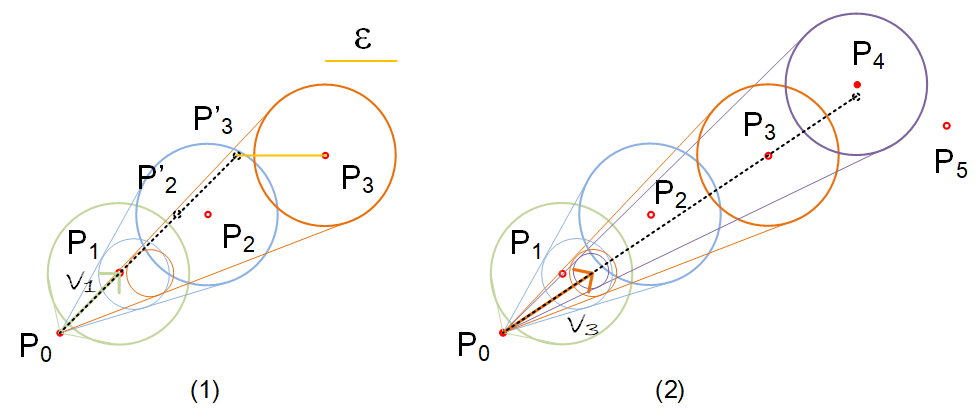
\includegraphics[scale=1.0]{figures/Fig-CITT.png}
	\vspace{-2ex}
	\caption{\small A running example of trajectory tracking by \citt. }
	\vspace{-3ex}
	\label{fig:citt}
\end{figure}


\begin{example}
	Figure~\ref{fig:citt} is a running example of algorithm \citt. It takes the same input and sets the same start point and initial velocity as Figure~\ref{fig:ldr}, and uses full-$\epsilon$ cones to simplify the trajectory. Then, (1) $P_3$ lives in the common intersection of \cone{_{1}} and \cone{_{2}} and it has a distance larger than $\epsilon$ to its expected position $P'_3$ \wrt $\vec{v_1}$, thus, \citt updates the velocity from $\vec{v_1}$ to $\vec{v_3}$ and the process goes on, and (2) $P_5$ is outside of the common intersection of the preview cones, thus, $P_4$ serves as the new start point, and an update is triggered. Finally, this algorithm sends three points, $P_0, P_4$ and $P_8$ (not shown), and four velocities, $\vec{v_1}$, $\vec{v_3}$, $\vec{v_5}$ (not shown) and $\vec{v_8}$ (not shown), to the MOD server. Also note that, no matter during the tracking or after the simplification, this algorithm ensures that any removed point is located in a circle around its expected position \wrt a velocity of trajectory tracking or a line segment connecting two neighboring data points of the simplified trajectory. 
\end{example}


\stitle{Correctness and complexity.} 
The correctness of algorithm \citt follows from Propositions \ref{theo-ldrh-cised} and \ref{theo-full-cone}.
It is easy to find that every point is processed only once in \citt, and for each point, it needs $O(1)$ time as getRPolygon() \cite{Lin:Cised}, intersecting of polygons \cite{Lin:Cised} and {other operations} all have a time complexity of $O(1)$. Hence, \citt has a time complexity of $O(n)$, where $n$ is the number of data points.






\eat{%%%%%%%%%%%%%%%%%%%%%%%%%%%%%%%%%%%%%%%%%%%%%%%%
	
\subsection{Weak tracking}

-- theorem: if ldr is true, then the intersection of those cones must not be \{$P_s$\}.
means that, if ldr is true, it is sure those points can be represented by a line segment.
thus, we only need to check the intersection after ldr is false, during the process.

-- algorithm CITT-W(e)

-- example

-- correctness and complexity
}%%%%%%%%%%%%%%%%%%%%%%%%%%%%%%%%%%%%%%%%%%%%%%%%%%%%%
